\chapter{Markov决策过程(MDP)}

\section{Markov决策过程的相关概念}

\subsection{Markov性}

Markov性是指一个随机过程未来发展的概率规律与观察之前的历史无关的性质。

如果$X(t),t>0$是一个随机过程,则Markov性指:
\begin{equation}
    \begin{aligned}
         & P\{X(t_{n+1})= x_{n+1}|X(t_n)=x_n,X(t_{n-1})=x_{n-1},\cdots,X(t_0) =x_0\} \\=&P\{X(t_{n+1})= x_{n+1}|X(t_n)=x_n\}
    \end{aligned}
\end{equation}

即系统未来的状态$x_{n+1}$只与当前状态$x_n$有关,而与历史状态$x_{n-1},x_{n-2},\cdots,x_0$无关。Markov性即状态转移概率的无后效性。

\subsection{Markov决策过程}

状态转移概率具有Markov性的随机过程即为Markov过程。

\begin{note}
    Markov决策过程又可看作随机对策的特殊情形,在这种随机对策中对策的一方是无意志的。Markov决策过程还可作为Markov型随机最优控制,其决策变量就是控制变量。
\end{note}

\subsubsection{Markov决策过程的基本要素}

Markov决策过程的基本要素包括:

\begin{enumerate}[itemsep=0pt,parsep=0pt]
    \item 阶段:$t=0,1,2,\cdots$,在一次决策过程中,每个阶段只能有一个决策,对应一个状态,所以下面的状态和阶段有时候表达同一个意思。
    \item 由于不同的决策,有时候相同阶段的状态不同。状态空间:$S=\{s_1,s_2,\cdots,s_n\}$。
    \item 决策者在每个阶段可采取的行动方案,决策空间:$A_{s_t}=\{a_1,a_2,\cdots,a_m\}$。
    \item 在一定决策下,系统经过一个阶段从某一状态转移到另一状态的可能性状态转移概率:$P_a(s_1,s_2)$。
    \item 每一阶段的成本:$g_{a_t}(s_t)$。
    \item 策略:根据当前时刻$t$和当前状态$s$,从可选行为集$A_{s_t}$中指定一个行为,记为$u$。
    \item 代价/奖励函数:衡量各方案好坏的指标,$J$。
\end{enumerate}

\begin{figure}[ht]
    \centering
    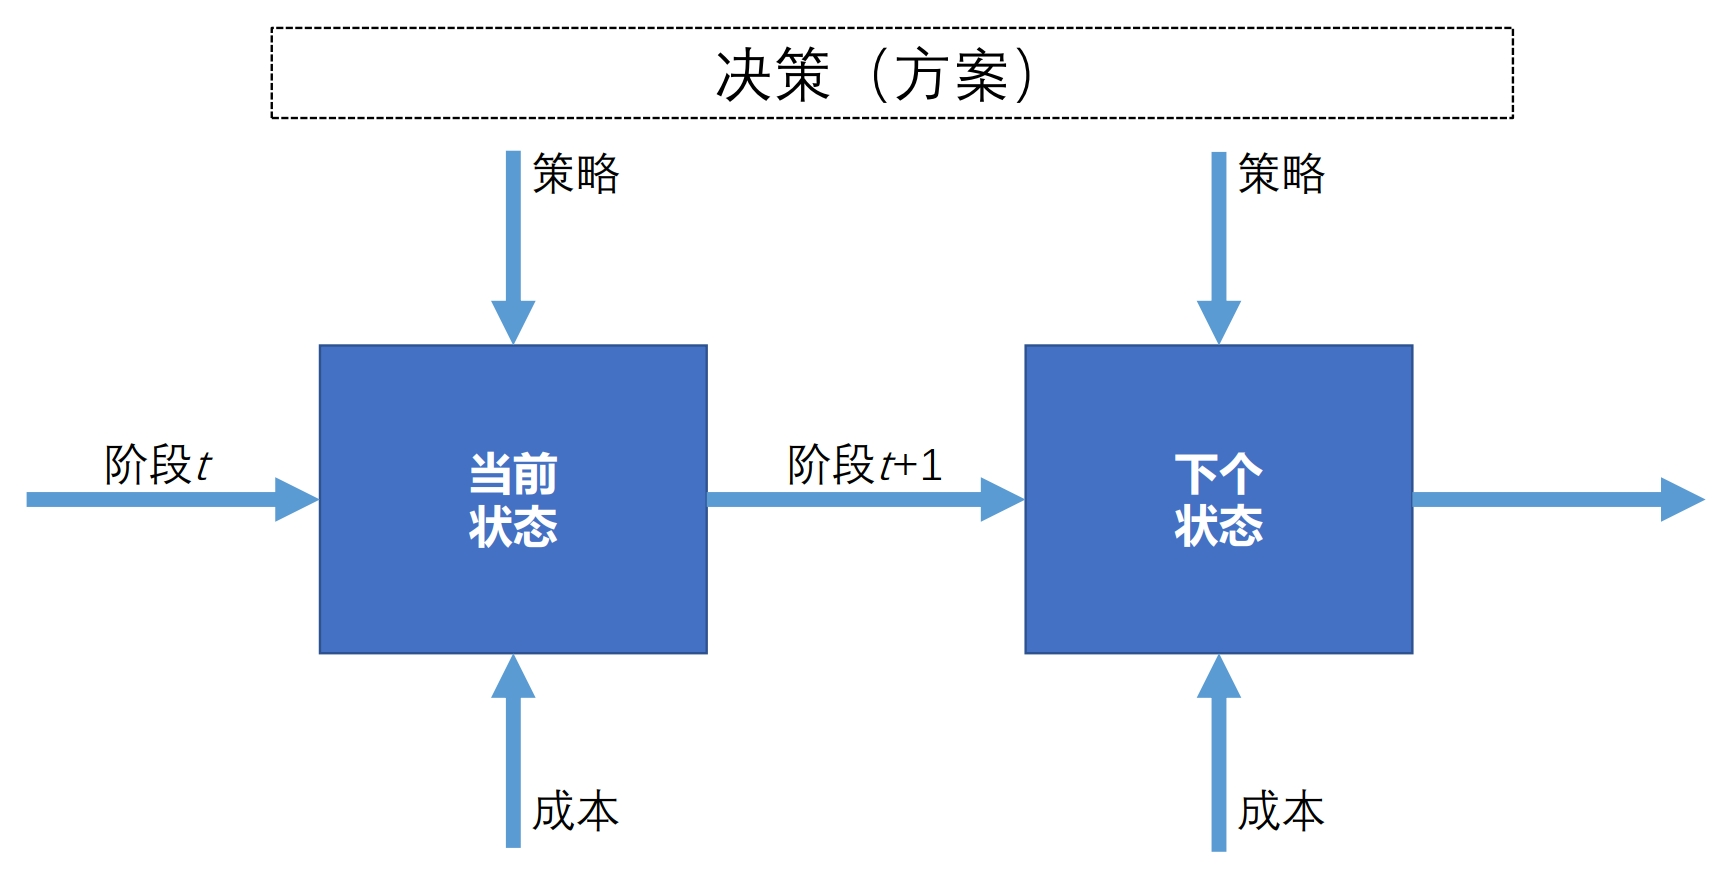
\includegraphics[width=0.8\textwidth]{pic/1.1.1.png}
    \caption{序列决策模型的过程示意}
\end{figure}

用新的符号集表示Markov性即为:

\begin{equation}
    \begin{aligned}
         & P\{S_{t+1}=s_{t+1}|S_t=s_t,A_t=a_t,S_{t-1}=s_{t-1},A_{t-1}\cdots,S_0=s_0\} \\=&P\{S_{t+1}=s_{t+1}|S_t=s_t,A_t=a_t\}
    \end{aligned}
\end{equation}

\subsubsection{Markov决策过程的表示方法}

系统方程:

\begin{equation}
    s_{t+1}=f(s_t,a_t,w_t)
\end{equation}

其中$w_t\in W$为随机扰动,$w_t$的分布与$t$无关,且与$s_t,a_t$无关。$t+1$时刻的状态$s_{t+1}$只与$t$时刻的状态$s_t$和$t$时刻的决策$a_t$有关。

转移概率矩阵:

\begin{equation}
    P_{a}(S_1,S_2)=P\{s_{t+1}=S_2|a_t=S_1,a_t=a\}
\end{equation}

给定当前状态为$s_t$,决策为$a_t$,则下一状态为$s_{t+1}$的概率为$P_{a_t}(s_t,s_{t+1})$。

一个Markov决策过程可以用一个四元组$(S,A,P,g)$来表示。

\begin{example}
    排队网络模型

    假设网络模型包括3台服务器, 2个不同的外部任务入口, 2条固定的工作流程1,2,3和4,5,6,7,8,在不同处理阶段的形成8个排队任务。

    \begin{figure}[ht]
        \centering
        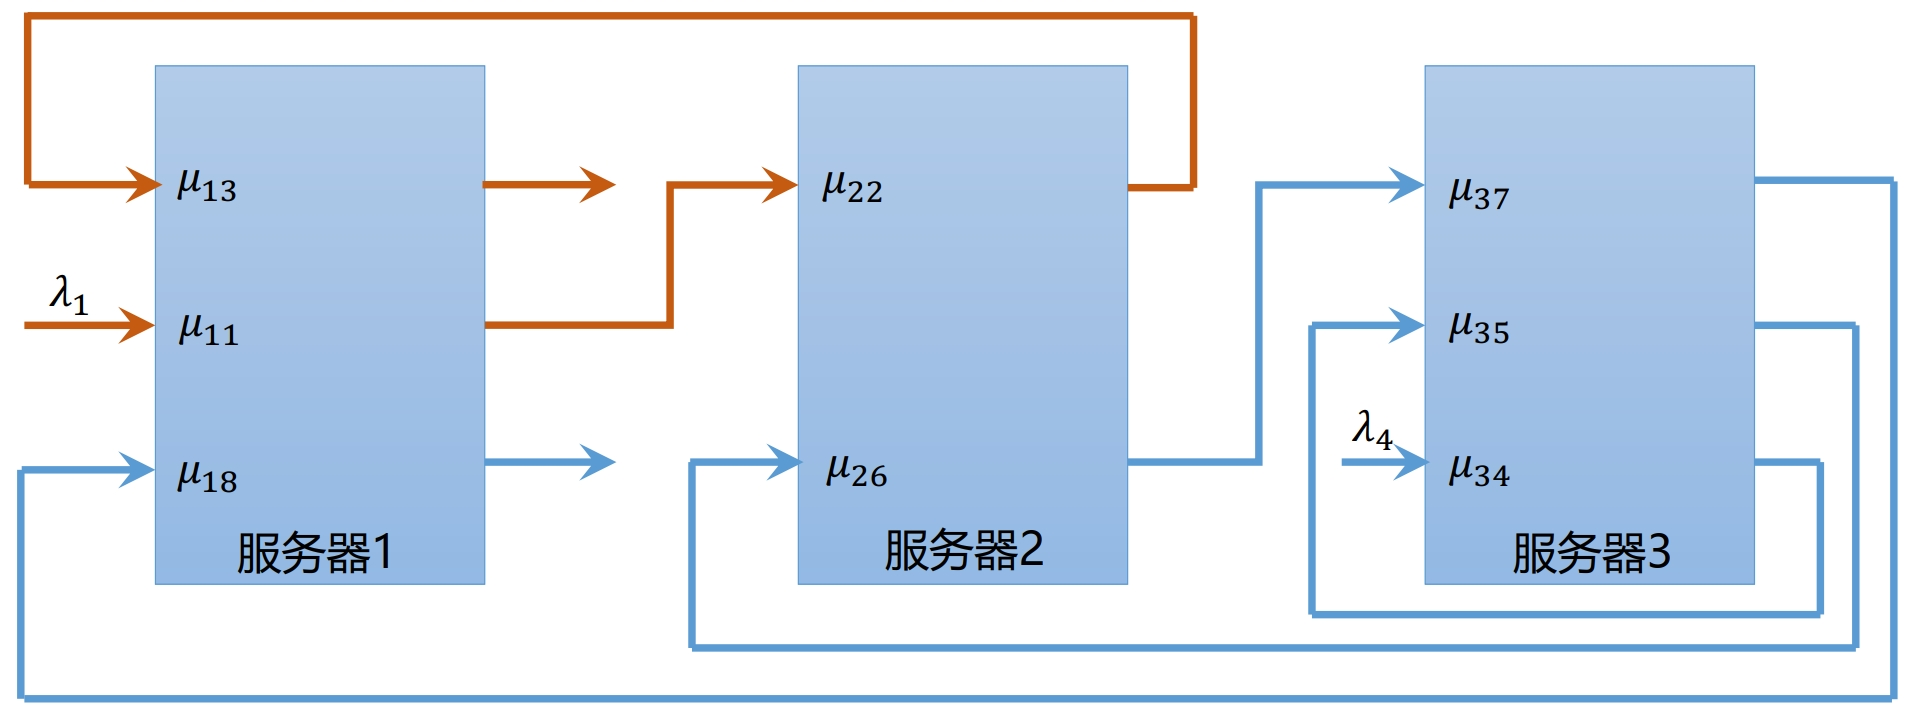
\includegraphics[width=0.8\textwidth]{pic/1.1.2.png}
        \caption{排队网络模型}
    \end{figure}

    我们假设服务时间满足几何随机变量:当服务器 $i$ 在一个时间步内服务于队列 $j$ 中的某一单元时,在本时间步内结束服务的概率为 $\mu _{ij}$,并独立于之前对该单元的服务。

    满足:
    \begin{enumerate}[itemsep=0pt,parsep=0pt]
        \item 任一时间步内,新的工作单元可以概率$\lambda_j$从队列$j=1,4$加入本系统;
        \item 新的工作单位独立于之前到达的工作单元;
        \item 某工作流程完成后, 此工作单元将被移送到整个流程的下一队列;
        \item 当所有流程已完成则该工作单元直接退出系该统。
    \end{enumerate}

    由于每个服务器都服务于多个队列,则在单个时间步内,必须选择确定服务器为哪个队列服务。这种选择可用八维向量代码$\alpha$编码,说明正接受服务的队列,并满足每个服务器只为单个队列服务的条件, 即$\alpha_i \in \{0,1\}$ ,且 $\alpha_1 +\alpha_3 +\alpha_8 \leq  1$,$\alpha_2 + \alpha_6 \leq 1$,$\alpha_4 + \alpha_5 + \alpha_7 \leq 1$。

    我们用对系统$x$的函数$u$来表述这个策略,该策略返回服务器工作分配情况。我们可用转移概率来表示队列的长度的变化——下一状态队列长度$x(t+1)$的条件概率由当前系统状态队列长度$x(t)$和决策$a(t)$确定,例如:

    到达队列1:
    \begin{equation}
        P(x_1(t+1)=x_1(t)+1|x_1(t),a(t))=\lambda_1
    \end{equation}

    离开队列1且到达队列2:
    \begin{equation}
        \begin{aligned}
             & P(x_1(t+1)=x_1(t)-1,x_2(t+1)=x_2(t)+1|x_1(t),x_2(t),a(t)) \\=&\mu_{11}I(x_1(t)>0,a_1(t)=1)
        \end{aligned}
    \end{equation}

    离开队列2且到达队列3:
    \begin{equation}
        \begin{aligned}
             & P(x_2(t+1)=x_2(t)-1,x_3(t+1)=x_3(t)+1|x_2(t),x_3(t),a(t)) \\=&\mu_{22}I(x_2(t)>0,a_2(t)=1)
        \end{aligned}
    \end{equation}

    离开队列3:
    \begin{equation}
        \begin{aligned}
            P(x_3(t+1)=x_3(t)-1|x_3(t),a(t))=\mu_{13}I(x_3(t)>0,a_3(t)=1)
        \end{aligned}
    \end{equation}

    其中$I(\cdot)$为指示函数,表示括号内条件为真时函数值为1,否则为0。


\end{example}

\subsubsection{最优准则}

最优准则——用以定义如何对不同时刻t的成本进行求和。

1. 有限阶段总成本:

\begin{equation}
    E[\sum_{t=0}^{T-1}g_{a_t}(s_t)|s_0=s]
\end{equation}

2. 平均成本:

\begin{equation}
    \lim_{T\rightarrow \infty}E[\frac{1}{T}\sum_{t=0}^{T-1}g_{a_t}(s_t)|s_0=s]
\end{equation}

3. 无限折扣成本:

\begin{equation}
    E[\sum_{t=0}^{\infty}\alpha^tg_{a_t}(s_t)|s_0=s]
\end{equation}

\begin{note}
    $\alpha \in (0,1)$ 是表示即时优先的折扣因子,特别的,当状态矢量空间和行为空间位有限集时, $ \bar{\alpha} < 1$足够大,从而对于所有的$\alpha > \bar{\alpha}$折扣成本问题的最优策略对于平均成本问题也是最优。

    采用折扣因子简化了分析和计算方法:数学表达上的方便、避免产生无限回报的情况、可以体现即时回报比延迟回报优先性。
\end{note}

\section{Markov决策过程的求解方法}

\subsection{有限阶段问题:逆推归纳法}

有限阶段内成本最小的策略,就是求解如下最优化问题:

\begin{equation}
    \min_{u_0,u_1,\cdots,u_{T-1}}E[\sum_{t=0}^{T-1}g_{a_t}(s_t)|s_0=s]
\end{equation}

动态规划的核心思想是:把方程改写成以下方程就可以大大简化寻求最优解的计算:
\begin{equation}
    \min_{a\in A_s}\left\{ g_a(x)+\sum_{s'\in S}P_a(s,s')\min_{u_1,\cdots,u_{T-1}}E[\sum_{t=1}^{T-1}g_{a_t}(s_t)|s_1=s']\right\}
\end{equation}

我们定义代价函数$J(s,t_0)$为从时刻$t_0$到时刻$T$的最优代价,即:
\begin{equation}
    J(s,t_0)=\min_{u_{t_0},\cdots,u_{T-1}}E[\sum_{t=t_0}^{T-1}g_{a_t}(s_t)|s_{t_0}=s]
\end{equation}

则有:
\begin{equation}
    J(s,t_0)=\min_{a\in A_s}\left\{ g_a(x)+\sum_{s'\in S}P_a(s,s')J(s',t_0+1)\right\}
\end{equation}

这是一个递归方程,从$J(s,T)=0$开始,逐步向前递推,直到$J(s,0)$,即可得到最优策略。

\begin{note}
    注意: 找到对应所有的$J(x,t)$需要大量的计算,计算量随着时间和状态的数量增大而线性增长,即使存在大量的呈指数增长的策略。
\end{note}

\begin{example}
    应急救援问题

    某应急救援车需要从$s$地出发到$t$地参与应急救援,期间的道路系统如下图所示,图中的圆圈表示途径的地方,连接两地的箭头表示道路,上面的数字表示该路段长度,箭头表示方向。试求$s$地到$t$地的最佳救援路线。

    \begin{figure}[ht]
        \centering
        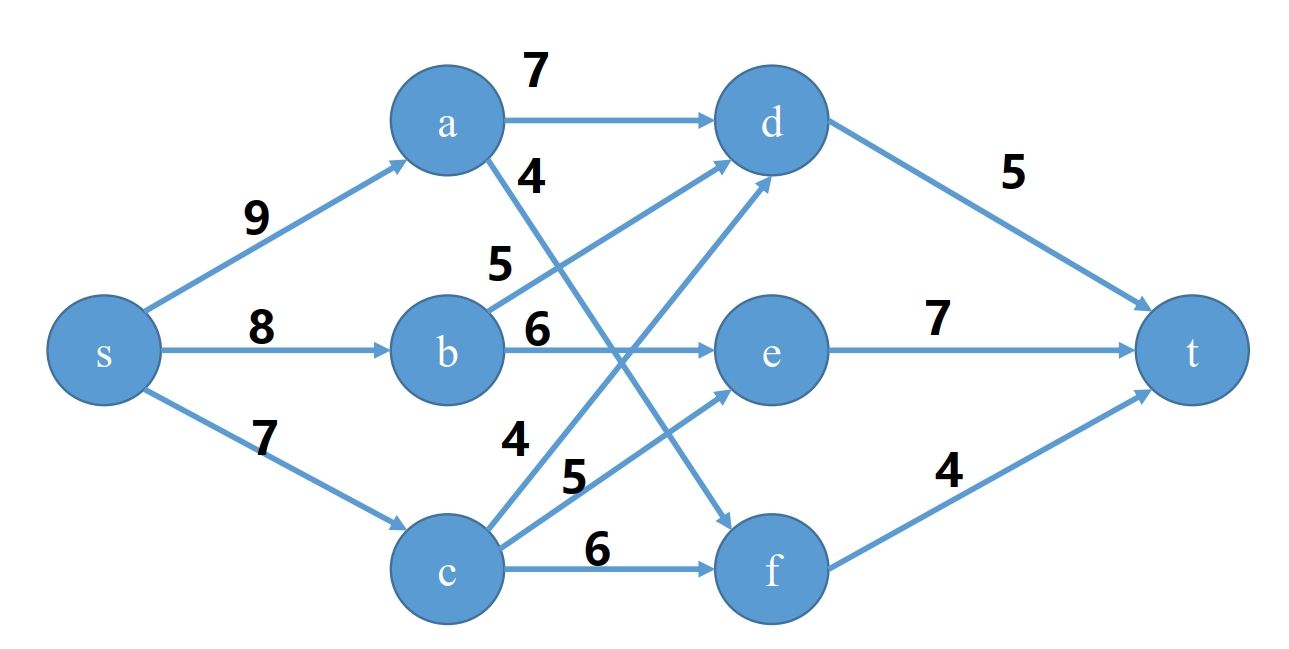
\includegraphics[width=0.8\textwidth]{pic/1.2.1.png}
        \caption{应急救援问题}
    \end{figure}

    \textbf{第一步:划分阶段}

    $k=1, 2, 3$表示三个阶段。

    \textbf{第二步:定义状态变量}

    状态变量$x_k$取为$k$阶段所在地,则有:
    \begin{equation}
        \begin{aligned}
            x_1 \in S_1 & = \{s\}
            x_2 \in S_2 & = \{a,b,c\} \\
            x_3 \in S_3 & = \{d,e,f\} \\
            x_4 \in S_4 & = \{t\}     \\
        \end{aligned}
    \end{equation}

    \textbf{第三步:定义策略和决策集}

    $k$阶段需要确定下一步走向哪里, $u_k(x_k)$即为$k$阶段, 状态为$x_k$时的策略:
    \begin{equation}
        \begin{aligned}
             & u_1 \in U_1 = \{a,b,c\}       \\
             & u_2(a) \in U_2(a) = \{d,f\}   \\
             & u_2(b) \in U_2(b) = \{d,e\}   \\
             & u_2(c) \in U_2(c) = \{d,e,f\} \\
             & u_3 \in U_3 = \{t\}           \\
        \end{aligned}
    \end{equation}

    \textbf{第四步:求解}

    根据有限阶段问题的逆推归纳法,可以逆序地求出条件最优代价函数值集合和条件最优策略集合。

    1.对第3阶段所有可能的状态$S_3 = \{d,e,f\}$ 计算条件最优代价函数值:

    第三阶段末已到达目的地,故$J_4(t) = 0$。
    \begin{equation}
        \begin{aligned}
            J_3(d) = \min_{u_3 \in U_3} \{g_{u_3}(d,t)+J_4(t)\} = 5 \\
            J_3(e) = \min_{u_3 \in U_3} \{g_{u_3}(e,t)+J_4(t)\} = 7 \\
            J_3(f) = \min_{u_3 \in U_3} \{g_{u_3}(f,t)+J_4(t)\} = 4 \\
        \end{aligned}
    \end{equation}
    其中$u_3(d) = u_3(e) = u_3(f) = t$。

    2.对第2阶段所有可能的状态$S_3 = \{a,b,c\}$ 计算条件最优代价函数值:

    \begin{equation}
        \begin{aligned}
            J_2(a) & = \min_{s_3 \in {d,f}} \{g_{u_2(a)}(a,s_3)+J_3(s_3)\}                                                                   \\
                   & =\min\left\{\begin{aligned} g_{u_2}(a,d)+ J_3(d) \\ g_{u_2}(a,f)+ J_3(f) \end{aligned} \right\}                         \\
                   & = \min\left\{\begin{aligned} 7+5 \\ 4+4 \end{aligned} \right\} =8                                                       \\
            J_2(b) & = \min_{s_3 \in {d,e}} \{g_{u_2(b)}(b,s_3)+J_3(s_3)\}                                                                   \\
                   & =\min\left\{\begin{aligned} g_{u_2}(b,d)+ J_3(d) \\ g_{u_2}(b,e)+ J_3(e) \end{aligned} \right\}                         \\
                   & = \min\left\{\begin{aligned} 5+5 \\ 6+7 \end{aligned} \right\} =10                                                      \\
            J_2(c) & = \min_{s_3 \in {d,e,f}} \{g_{u_2(c)}(c,s_3)+J_3(s_3)\}                                                                 \\
                   & =\min\left\{\begin{aligned} g_{u_2}(c,d)+ J_3(d) \\ g_{u_2}(c,e)+ J_3(e) \\ g_{u_2}(c,f)+ J_3(f) \end{aligned} \right\} \\
                   & = \min\left\{\begin{aligned} 4+5 \\ 5+7 \\ 6+4 \end{aligned} \right\} =9                                                \\
        \end{aligned}
    \end{equation}
    其中$u_2(a) = d$,$u_2(b) = d$,$u_2(c) = c$。

    类似求解第一阶段,可以得到$s\rightarrow c\rightarrow d\rightarrow t$:

    \begin{figure}[ht]
        \centering
        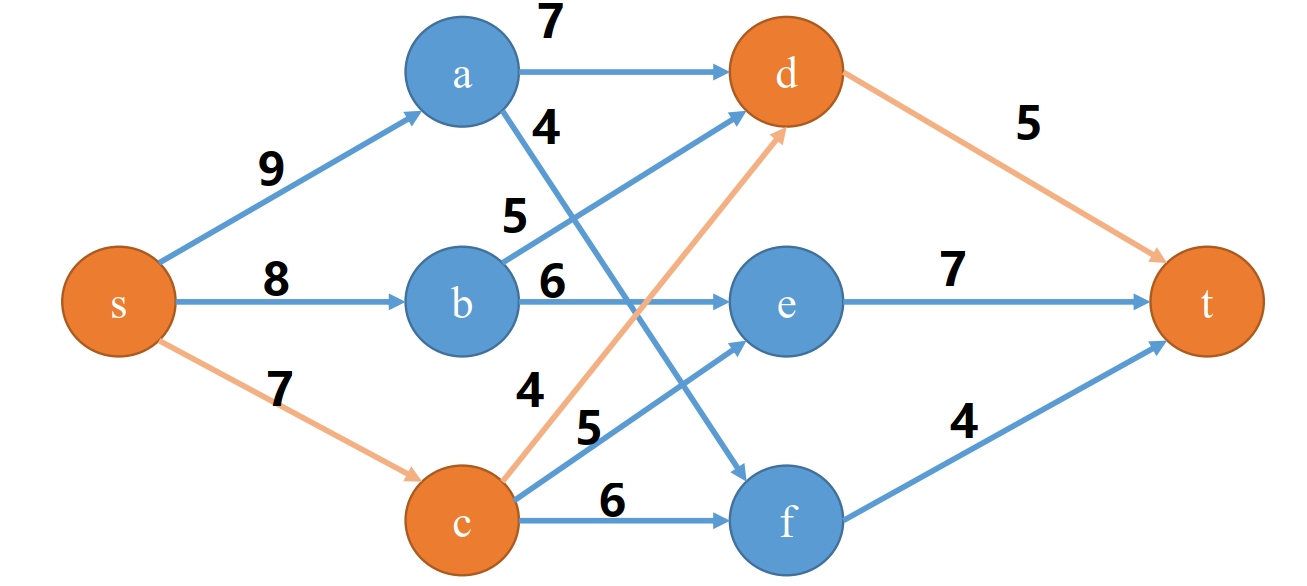
\includegraphics[width=0.8\textwidth]{pic/1.2.2.png}
        \caption{应急救援问题的最优策略}
    \end{figure}

\end{example}

\subsection{折扣成本问题:Bellman方程}

\subsubsection{代价函数与Bellman方程}

同上面的有限阶段问题类似,我们可以定义折扣成本问题的条件最优代价函数值:
\begin{equation}
    J(s,t_0)=\min_{u\in U}E[\sum_{t=t_0}^{\infty}\alpha^{t-t_0}g_{a_t}(s_t)|s_{t_0}=s]
    \label{eq:1.2.1}
\end{equation}

则有:
\begin{equation}
    J(s,t_0)=\min_{a\in A_s}\left\{ g_a(x)+\alpha\sum_{s'\in S}P_a(s,s')J(s',t_0+1)\right\}
\end{equation}

对于无限范围的情况,由\ref{eq:1.2.1}可知,对于任意的$t$和$t'$,总有$J(s,t)=J(s,t')$,即$J(s,t)$与$t$无关,我们可以将其简写为$J(s)$。

这是因为:
\begin{equation}
    \begin{aligned}
        J(s,t) & = \min_{u\in U}E[\sum_{t=t_0}^{\infty}\alpha^{t-t_0}g_{a_t}(s_t)|s_{t_0}=s]    \\
               & = \sum_{t=t_0}^{\infty}\alpha^{t-t_0}P_u(s_{t_0}=s,s_t=\sigma)g_u(s)(\sigma)   \\
               & = \sum_{t=t_0}^{\infty}\alpha^{t-t_0}P_u(s_{t-t_0}=s,s_0=\sigma)g_u(s)(\sigma) \\
               & = \sum_{t=0}^{\infty}\alpha^{t}P_u(s_{t}=s,s_0=\sigma)g_u(s)(\sigma)           \\
    \end{aligned}
\end{equation}
是一个和$t$无关的数。其中$\sigma$为最终状态,转移矩阵与$t$无关。也可以通过无后效性来理解。

同样地$u$也与$t$无关,称为平稳策略。我们给出了Bellman方程的最终形式:

\begin{equation}
    J(s)=\min_{a\in A_s}\left\{ g_a(x)+\alpha\sum_{s'\in S}P_a(s,s')J(s')\right\}
\end{equation}

\subsubsection{动态规划算子}

对于每一个平稳策略$u$,我们用$g_u$表示元项为$g_{u_x}(x)$的矢量,$P_u$表示元项为$P_{u_x}(x)$的矩阵。现在来定义动态规划算子$T$和$T_u$。

我们可以将Bellman方程写成算子的形式:
\begin{equation}
    T_uJ=g_u+\alpha P_uJ
\end{equation}
\begin{equation}
    TJ=\min_{u\in U}T_uJ
\end{equation}
其中$J$是一个向量,记录每一个状态的最优代价函数值。

从而有:
\begin{equation}
    J=TJ
\end{equation}

一般来讲,对于任意函数$J$,若$T_uJ=TJ$ 则认为策略$u$是与$J$强相关。我们把与$J$强相关的策略记为$u_J$,即$u_J$是$T_uJ=TJ$的解。

\begin{note}
    例如$T_{u_{J_{u_{k}}}}$。

    $u_{k}$: 可选行为集中的某一策略;

    $J_{u_{k}}$: 以$u_{k}$为策略时的代价函数;

    $u_{J_{u_{k}}}$: 以$u_{k}$强相关的策略;

    $T_{u_{J_{u_{k}}}}$: 以$u_{J_{u_{k}}}$为策略时的动态规划算子。
\end{note}

动态规划算子的三大特性: 单调性、 偏移性、 最大模收缩

\begin{enumerate}[itemsep=0pt,parsep=0pt]
    \item 单调性: 若$J_1\leq J_2$,则$TJ_1\leq TJ_2$。
    \item 偏移性: 对于所有的$J$和属于R的常数$c$,有$T(J+ce)=TJ+\alpha ce$。
    \item 最大模收缩: $\|TJ_1-TJ_2\|_{\infty}\leq \alpha \|J_1-J_2\|_{\infty}$。
\end{enumerate}

证明:

1. 单调性:

\begin{equation}
    \begin{aligned}
        TJ_1\leq T_{u_{J_2}}J_1 & = g_{u_{J_2}}+\alpha P_{u_{J_2}}J_1    \\
                                & \leq g_{u_{J_2}}+\alpha P_{u_{J_2}}J_2 \\
                                & = T_{u_{J_2}}J_2                       \\
                                & \leq TJ_2                              \\
    \end{aligned}
\end{equation}

2. 偏移性:

\begin{equation}
    \begin{aligned}
        T(J+ce) & = \min_{u\in U}T_u(J+ce)          \\
                & = \min_{u\in U}T_uJ+\alpha cP_u e \\
                & = TJ+\alpha ce                    \\
    \end{aligned}
\end{equation}

3. 最大模收缩:


注意到:
\begin{equation}
    \begin{aligned}
        J = J + J' - J' \leq J' + \|J-J'\|_{\infty}e
    \end{aligned}
\end{equation}


\begin{equation}
    \begin{aligned}
        TJ - TJ'            & = T(J-J')                            \\
                            & \leq T(J' + \|J-J'\|_{\infty}e - J') \\
                            & = \alpha \|J-J'\|_{\infty}e          \\
        \|TJ-TJ'\|_{\infty} & \leq \alpha \|J-J'\|_{\infty}
    \end{aligned}
\end{equation}
其中用到了前两条性质。

\subsection{数值迭代方法}

\subsubsection{Bellman方程解的唯一性}

对于Bellman方程,我们可以通过迭代的方法求解。我们可以从任意的$J_0$开始,通过$J_{k+1}=TJ_k$来迭代求解。

我们先证明Bellman方程的解的存在唯一性。

\begin{proof}
    1. 存在性:

    由于$T$是一个压缩映射,所以$T$有唯一不动点,即$TJ=J$有唯一解$J^*$。

    2. 唯一性:

    假设$J_1$和$J_2$都是Bellman方程的解,则有:
    \begin{equation}
        \begin{aligned}
            J_1 & = T J_1 \\
            J_2 & = T J_2 \\
        \end{aligned}
    \end{equation}

    从而有:
    \begin{equation}
        \begin{aligned}
            \|J_1-J_2\|_{\infty} & = \|TJ_1-TJ_2\|_{\infty}         \\
                                 & \leq \alpha \|J_1-J_2\|_{\infty}
        \end{aligned}
    \end{equation}

    由于$\alpha < 1$,所以$J_1=J_2$。
\end{proof}

这就说明数值迭代方法是收敛的,一定可以找到Bellman方程的解。而且解是唯一的。

\begin{example}

    段数不定的最短路线问题(不定期决策过程)

    $n$个点相互连接组成 一个连通图(图中$n=5$),各点标号为$1,2,…, n$ 。任意两点$i,j$之间的距离(费用)记作$d_{ij}$ 。求任意一点$i$到点$n$(靶点)的最短路线(距离)。

    \begin{figure}[ht]
        \centering
        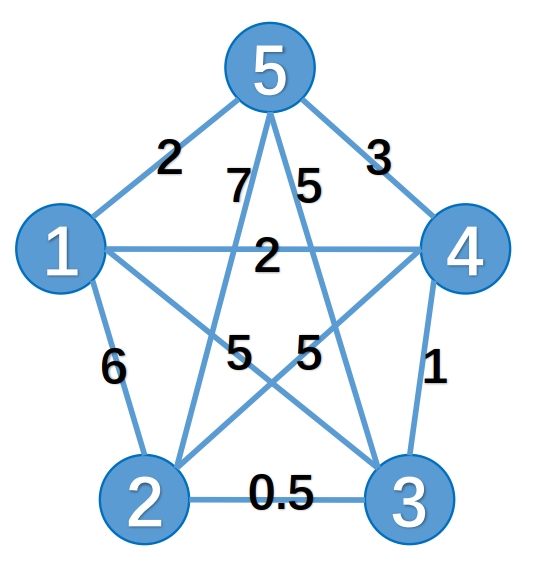
\includegraphics[width=0.4\textwidth]{pic/1.2.3.png}
        \caption{段数不定的最短路线问题}
    \end{figure}

    1.从$i$点走一步到靶点5的最优距离为$J_1(i)$ , 则显然有:
    \begin{equation}
        J_1(i)=d_{i5}
    \end{equation}
    具体说:
    \begin{equation}
        \begin{aligned}
            J_1(1) & = d_{15} = 2 \\
            J_1(2) & = d_{25} = 7 \\
            J_1(3) & = d_{35} = 5 \\
            J_1(4) & = d_{45} = 3 \\
            J1(5)  & = d_{55} = 0 \\
        \end{aligned}
    \end{equation}

    其中最优决策为:
    \begin{equation}
        u_1(i)=\arg \min_{j\in N(i)}\{d_{ij}\}
    \end{equation}
    具体说:
    \begin{equation}
        \begin{aligned}
            u_1(1) & = 5 \\
            u_1(2) & = 5 \\
            u_1(3) & = 5 \\
            u_1(4) & = 5 \\
            u_1(5) & = 5 \\
        \end{aligned}
    \end{equation}

    2.从$i$点走两步到靶点5的最优距离为为$J_2(i)$ , 根据最优化原理得:

    \begin{equation}
        J_2(i)=\min_{j\in N(i)}\{d_{ij}+J_1(j)\}
    \end{equation}
    具体说:
    \begin{equation}
        \begin{aligned}
            J_2(1) & = \min\{d_{11}+J_1(1),d_{12}+J_1(2),d_{13}+J_1(3),d_{14}+J_1(4),d_{15}+J_1(5)\} \\
                   & = \min\{0+2,6+7,5+5,2+3,2+0\}                                                   \\
                   & = 2                                                                             \\
            J_2(2) & = \min\{d_{21}+J_1(1),d_{22}+J_1(2),d_{23}+J_1(3),d_{24}+J_1(4),d_{25}+J_1(5)\} \\
                   & = \min\{6+2,0+7,0.5+5,5+3,7+0\}                                                 \\
                   & = 5.5                                                                           \\
            J_2(3) & = \min\{d_{31}+J_1(1),d_{32}+J_1(2),d_{33}+J_1(3),d_{34}+J_1(4),d_{35}+J_1(5)\} \\
                   & = \min\{5+2,0.5+7,0+5,1+3,5+0\}                                                 \\
                   & = 3                                                                             \\
            J_2(4) & = \min\{d_{41}+J_1(1),d_{42}+J_1(2),d_{43}+J_1(3),d_{44}+J_1(4),d_{45}+J_1(5)\} \\
                   & = \min\{2+2,5+7,1+5,0+3,3+0\}                                                   \\
                   & = 3                                                                             \\
            J_2(5) & = \min\{d_{51}+J_1(1),d_{52}+J_1(2),d_{53}+J_1(3),d_{54}+J_1(4),d
            _{55}+J_1(5)\}                                                                           \\
                   & = 0                                                                             \\
        \end{aligned}
    \end{equation}

    其中最优决策为:
    \begin{equation}
        u_2(i)=\arg \min_{j\in N(i)}\{d_{ij}+J_1(j)\}
    \end{equation}
    具体说:
    \begin{equation}
        \begin{aligned}
            u_2(1) & = 5 \\
            u_2(2) & = 3 \\
            u_2(3) & = 4 \\
            u_2(4) & = 5 \\
            u_2(5) & = 5 \\
        \end{aligned}
    \end{equation}

    3.从$i$点走三步到靶点5的最优距离为为$J_3(i)$ , 根据最优化原理得:

    按照同样的方法解得:
    \begin{equation}
        \begin{aligned}
            J_3(1) & = 2   \\
            J_3(2) & = 4.5 \\
            J_3(3) & = 4   \\
            J_3(4) & = 3   \\
            J_3(5) & = 0   \\
        \end{aligned}
    \end{equation}
    \begin{equation}
        \begin{aligned}
            u_3(1) & = 5 \\
            u_3(2) & = 3 \\
            u_3(3) & = 4 \\
            u_3(4) & = 5 \\
            u_3(5) & = 5 \\
        \end{aligned}
    \end{equation}

    4.从$i$点走四步到靶点5的最优距离为为$J_4(i)$ , 根据最优化原理得:

    按照同样的方法解得:
    \begin{equation}
        \begin{aligned}
            J_4(1) & = 2   \\
            J_4(2) & = 4.5 \\
            J_4(3) & = 4   \\
            J_4(4) & = 3   \\
            J_4(5) & = 0   \\
        \end{aligned}
    \end{equation}
    \begin{equation}
        \begin{aligned}
            u_4(1) & = 5 \\
            u_4(2) & = 3 \\
            u_4(3) & = 4 \\
            u_4(4) & = 5 \\
            u_4(5) & = 5 \\
        \end{aligned}
    \end{equation}
    数值稳定,说明迭代完成。

    下面是示例代码:

\end{example}

\begin{lstlisting}[language=python]
import numpy as np

def compute_shortest_paths(n, distances):
"""
计算最短路径的函数。

参数:
n -- 点的个数
distances -- 二维数组,表示每两点之间的距离

返回:
J -- 每个点到目标点的最短路径长度
u -- 每个点到目标点的最优决策路径
"""
# 初始化J和u数组。J记录最短路径长度,u记录最优决策路径。
J = np.zeros((n, n))
u = np.zeros((n, n), dtype=int)

# 初始条件:从每个点到目标点n的直接距离
for i in range(n):
J[i][0] = distances[i][n-1]
u[i][0] = n

# 进行k步迭代,计算每个点通过k步到达目标点的最短路径
for k in range(1, n):
for i in range(n):
# 计算通过中间点到达目标点的最短距离
min_distance = float('inf')
for j in range(n):
distance = distances[i][j] + J[j][k-1]
if distance < min_distance:
min_distance = distance
u[i][k] = j + 1  # 存储最优决策点
J[i][k] = min_distance

return J, u

# 假设的距离矩阵,这里需要具体的距离数据来填充
n = 5  # 点的数量
distances = np.array([
        [0, 6, 5, 2, 2],
        [6, 0, 0.5, 5, 7],
        [5, 0.5, 0, 1, 5],
        [2, 5, 1, 0, 3],
        [2, 7, 5, 3, 0]
    ])

# 计算最短路径
J, u = compute_shortest_paths(n, distances)
\end{lstlisting}

\subsubsection{Gauss-Seidel迭代}

\href{https://en.wikipedia.org/wiki/Gauss%E2%80%93Seidel_method}{Gauss-Seidel迭代}是一种特殊的数值迭代方法,它的特点是每次迭代都是在实时更新的结果上进行的,而不是像一般的迭代方法那样,每次迭代都是在上一次迭代的结果上进行的。

不同于上面的Jacobi迭代,Gauss-Seidel迭代是一种逐点更新的方法,即每次更新一个点,而不是一次更新所有点。这样的好处是可以节省内存,因为每次只需要存储一个点的值,而不是所有点的值。

如果$A=D+L+U$,其中$D$是$A$的对角矩阵,$L$是$A$的严格下三角矩阵,$U$是$A$的严格上三角矩阵,则普通的Jacobi迭代可以写成:
\begin{equation}
    Dx^{(k+1)}=b-(L+U)x^{(k)}
\end{equation}
其中$x^{(k)}$是第$k$次迭代的结果,$b$是方程组$Ax=b$的右端项。

如果我们写出$Ax=b$的每一行,第$i$行为:
\begin{equation}
    \sum_{j=1}^{n}a_{ij}x_j=b_i
\end{equation}

对这一行的求解为:
\begin{equation}
    x_i^{({\color{red}k+1})}=\frac{1}{a_{ii}}(b_i-\sum_{j=1}^{i-1}a_{ij}x_j^{({\color{red}k})}-\sum_{j=i+1}^{n}a_{ij}x_j^{({\color{red}k})})
\end{equation}

如果$A=D+L+U$,其中$D$是$A$的对角矩阵,$L$是$A$的严格下三角矩阵,$U$是$A$的严格上三角矩阵,则Gauss-Seidel迭代可以写成:
\begin{equation}
    (D+K)x^{(k+1)}=b-Ux^{(k)}
\end{equation}

对应的迭代形式为:
\begin{equation}
    x_i^{({\color{red}k+1})}=\frac{1}{a_{ii}}(b_i-\sum_{j=1}^{i-1}a_{ij}x_j^{({\color{red}k+1})}-\sum_{j=i+1}^{n}a_{ij}x_j^{({\color{red}k})})
\end{equation}

Jacobi 迭代和 Gauss-Seidel 迭代形式几乎一样。但 Gauss-Seidel 及时利用了最新的迭代结果,直观上比 Jacobi 效率更高。\footnote{这一段论述来源于\href{https://zhuanlan.zhihu.com/p/389389672}{知乎},其中给出了很详细的解释和图示。}

我们可以定义新的算符:

\begin{equation}
    FJ(x)=\min_{u\in U}\left\{ g_u(x)+\alpha\sum_{y<x}P_u(x,y)FJ(y)+\alpha \sum_{y\geq x}P_U(x,y)J(y)\right\}
\end{equation}

同样地,这样的算符也是压缩映射,不动点也为Bellman方程的解$J^*$。

\subsection{平稳策略的最优化}

从一个引理出发:

\begin{quotation}

    如果$J\leq TJ$,则$J\leq J^*$; 如果$J\geq TJ$,则$J\geq J^*$。其中$J^*$为Bellman方程的解。

\end{quotation}


该引理利用迭代显然。

而对于平稳策略,就有以下的性质:

\begin{quotation}

    $u\in U$表示任意策略,$u^*=u_{J^*}$是最优策略(有$J^*=TJ^*=T_{u^*}J^*$),则有:$J_u\geq J_{u^*}=J^*$。如果$u$为满足$T_uJ^*\neq TJ^*$的任意策略,则至少存在一个状态$x$,使得$J_u(x)>J^*(x)$。

\end{quotation}

\begin{proof}
    先说明$J_{u^*}=J^*$。

    由于$J^*=TJ^*=T_{u^*}J^*$,所以$J^*$是$T_{u^*}$的不动点,而$T_{u^*}$是压缩映射,所以$J^*$是唯一的不动点,即$J_{u^*}=J^*$。

    对于其他任何策略,都有$J_u\geq TJ_u$,所以$J_u\geq TJ_u\geq TJ^*=J^*$。

    考虑平稳策略$u$,如果$T_uJ^*\neq TJ^*$,即$T_uJ^*\geq TJ^*$,并存在至少一个状态$x$,使得$T_uJ^*(x)>TJ^*(x)$,则有:
    \begin{equation}
        \begin{aligned}
            J_u(x) & \geq T_uJ^*(x) > TJ^*(x) = J^*(x)
        \end{aligned}
    \end{equation}
\end{proof}

\begin{example}
    折扣成本相关例题分析:

    某地A发生了一场地震,为了尽快进行灾后救援,政府需要从灾区外某地B向灾区运送救援物资,而地震后五天内的救援是十分重要的。因此,我们模拟一个向震区运送物资的情景,并考虑如何在五天内运送尽可能多的物资。

    假设从B地前往A地的道路大多被地震破坏封堵,眼下还有两条路径,分别标记为M和N, B地一共有$1000$辆汽车可用于物资运输,并且通过M、 N路径前往A地往返一次都只需要一天的时间。M路受地震影响较小,路况较好,汽车往返一次不发生故障的概率$\beta= 0.9$, 但是M路需要通过一座受过地震影响的桥梁,为了保障桥梁的安全, M路上的汽车载重不能超过$5$吨。N路不需要通过这样的桥梁,汽车可以满载$8$吨,但是由于N路受地震影响较大,路况较差,往返一次后车辆不发生故障的概率$\alpha = 0.7$。

    在这紧张的五天内,每天晚上都会对所有的汽车进行检修, 若没有发生故障可以将汽车状态恢复如初;一旦发生故障,简单的检修不足以让该车辆在五天内恢复正常工作.假设发生故障的汽车可以顺利完成本次运输任务并成功返回B地。

    显然,分配不同数目的车辆分别从M、 N两条路同时向灾区运送物资才能在五天内运送更多的物资,而如何分配两条路上车辆的比例则是我们需要解决的问题。

    \textbf{问题分析}

    从假设中可以看出,五天内的分配策略之间是无后效性的,可以考虑用Markov决策过程进行分析。

    首先对此过程进行一些假设:

    设阶段$k$表示天数,则$k = 1,2,3,4,5$;状态变量$S_k$表示第$k$天初所拥有的未发生故障的车辆数目,亦即$k-1$天晚上未发生故障的车辆数目;决策变量$x_k$表示在第$k$天分配从N路前往灾区的车辆数目,同时得到$S_k-x_k$为当日分配从M路前往灾区的车辆数目。

    可得状态转移方程为:
    \begin{equation}
        S_{k+1} = \alpha x_k+\beta(S_k-x_k) = 0.9S_k-0.2x_k
    \end{equation}

    允许决策的集合为:
    \begin{equation}
        U_k = \{x_k\in \mathbb{N} | 0\leq x_k\leq S_k\}
    \end{equation}

    设一个阶段指标$g_k(S_k, x_k)$作为每个阶段向灾区运送的物资总和:
    \begin{equation}
        g_k(S_k, x_k) = 8x_k+5(S_k-x_k) = 5S_k+3x_k
    \end{equation}

    设有最优函数$J_k(S_k)$表示从现有的资源$S_k$出发,采取最优策略向灾区运送的物资总量,可以得到Bellman方程:
    \begin{equation}
        \begin{aligned}
            J_k(S_k) & = \max_{x_k\in U_k}\{g_k(S_k, x_k)+ J_{k+1}(S_{k+1})\}  \\
                     & = \max_{x_k\in U_k}\{5S_k+3x_k+J_{k+1}(0.9S_k-0.2x_k)\}
        \end{aligned}
    \end{equation}
    对于边界情况我们有: $J_6(S_6) = 0$。

    在$k= 5$时:
    \begin{equation}
        \begin{aligned}
            J_5(S_5) & = \max_{x_5\in U_5}\{5S_5+3x_5+J_6(S_6)\} \\
                     & = \max_{x_5\in U_5}\{5S_5+3x_5\}
        \end{aligned}
    \end{equation}
    是关于$S_5$的线性函数,其最优策略为$x_5^* = S_5$,最优值为$J_5^*(S_5) = 8S_5$。

    在$k= 4$时:
    \begin{equation}
        \begin{aligned}
            J_4(S_4) & = \max_{x_4\in U_4}\{5S_4+3x_4+J_5(0.9S_4-0.2x_4)\} \\
                     & = \max_{x_4\in U_4}\{5S_4+3x_4+8(0.9S_4-0.2x_4)\}   \\
                     & = \max_{x_4\in U_4}\{12.2S_4+1.4x_4\}
        \end{aligned}
    \end{equation}
    是关于$S_4$的线性函数,其最优策略为$x_4^* = S_4$,最优值为$J_4^*(S_4) = 13.6S_4$。

    以此类推,可以得到:

    $k= 3$时,$J_3^*(S_3) = 17.5S_3$,$x_3^* = S_3$;

    $k= 2$时,$J_2^*(S_2) = 20.8S_2$,$x_2^* = 0$;

    $k= 1$时,$J_1^*(S_1) = 23.7S_1$,$x_1^* = 0$。

    计算结果表明,最优策略为前两天将车辆全部安排从M路走,后三天将全部车辆安排从N路行驶,这样可以实现$5$天内运输的物资数目最大,最大的运量为$23700$吨。由此也可以根据最优策略得出每个阶段的状态,我们可以据此阶段顺序来分别计算每天完好车辆数量:
    \begin{equation}
        \begin{aligned}
            S_1 & = 1000                \\
            S_2 & = 0.9S_1-0.2x_1 = 900 \\
            S_3 & = 0.9S_2-0.2x_2 = 810 \\
            S_4 & = 0.9S_3-0.2x_3 = 567 \\
            S_5 & = 0.9S_4-0.2x_4 = 397 \\
            S_6 & = 0.9S_5-0.2x_5 = 278 \\
        \end{aligned}
    \end{equation}

\end{example}


\subsection{策略迭代}

策略迭代算法过程如下:

\begin{enumerate}[itemsep=0pt,parsep=0pt]
    \item 以策略$u_0$,$k=0$开始;
    \item 代价评估阶段:计算$J_{u_k} = g_{u_k}+\alpha P_{u_k}J_{u_k}$;
    \item 策略改善阶段:选择$u_{k+1} = u_{J_{u_k}}$;
    \item 如果$u_{k+1} = u_k$,则停止,否则令$k=k+1$,转到步骤2。
\end{enumerate}

\begin{note}
    步骤2是为每一次迭代获得更佳的策略。由于策略集是有限的,该算法将在有限的时间步内终止,我们通常用下述定理正式阐述这种概念。
\end{note}

\begin{quote}
    经过有限次迭代后,策略迭代收敛于$u^*$,即$u_k=u^*$,并且$J_{u_k}=J^*$。
\end{quote}

\begin{proof}
    若$u_k$是最优的,即得证。

    否则,存在一个状态$x$,使得$T J_{u_k} <= T_{u_k}J_{u_k} < J_{u_k}$。

    由于$T_{u_{k+1}}J_{u_k} = T_{u_{J_{u_k}}}J_{u_k} = TJ_{u_k}$,且$J_{u_k}=T_{u_k}J_{u_k}$,所以$J_{u_k} = T_{u_{k}}J_{u_k} >= TJ_{u_k} = T_{u_{k+1}}J_{u_k} >= T^n_{u_{k+1}}J_{u_k} \rightarrow J_{u_{k+1}}$。

    因此,策略$u_{k+1}$比策略$u_k$更优,与假设矛盾。
\end{proof}

对于数值迭代步骤:

\begin{enumerate}[itemsep=0pt,parsep=0pt]
    \item $J_0, k = 0$;
    \item $J_{k+1} = T J_k, k = k+1$;
    \item 若$J_{k+1} - J_k < \epsilon$,迭代结束,否则返回步骤2。
\end{enumerate}

数值迭代法和策略迭代法中, 序列$J_j$和$u_k$的收敛性在相当广泛的条件下是可以保证的,一般来说它与状态$S$、 决策$A_{x_t}$ 、状态转移概率 $P_a(x,y)$等的具体形式有关。

\textbf{数值迭代法}的基本思想是:以步数(段数)作为参数,以代价函数作为参考值,先求在各个不同步数下的最优策略,然后从这些最优解中再选出最优者,从而同时确定了最优步数。

\textbf{策略迭代法}的基本思想是:先选定一初始策略$u_0$, 然后按某种方式求得新策略,直至最终求出最优策略。若对某一$k$, 对所有阶段有: $u_{k+1}=u_k$,则称策略收敛,此时, 策略$u_k$就是最优策略。

下面用策略迭代方法重新求解上面的问题:

\begin{example}

    段数不定的最短路线问题(不定期决策过程)

    $n$个点相互连接组成 一个连通图(图中$n=5$),各点标号为$1,2,…, n$ 。任意两点$i,j$之间的距离(费用)记作$d_{ij}$ 。求任意一点$i$到点$n$(靶点)的最短路线(距离)。

    \begin{figure}[ht]
        \centering
        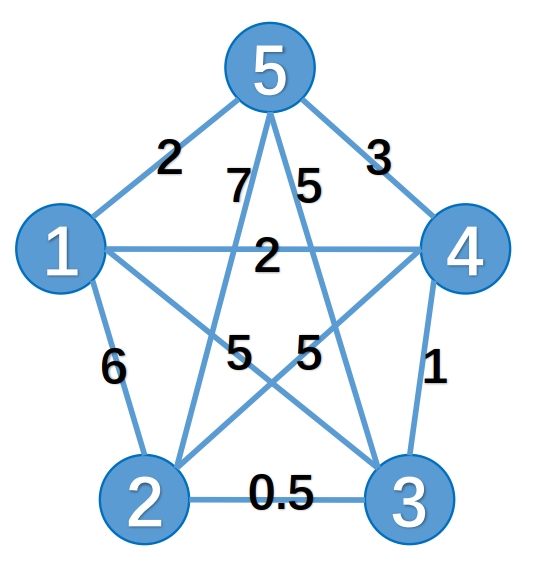
\includegraphics[width=0.4\textwidth]{pic/1.2.3.png}
        \caption{段数不定的最短路线问题}
    \end{figure}

    \textbf{第一步}

    \textbf{1.}

    先选取初始策略$u_1(i)$,例如取$u_1(1)=5,u_1(2)=4,u_1(3)=5,u_1(4)=3$,即$U_1=\{5,4,5,3\}$。注意必须无回路,每点可达靶点。

    \textbf{2.}

    由$u_1$可得$J_1(i)$,由策略迭代法可得:
    \begin{equation}
        \begin{aligned}
            J_1(i) & = d_{i,u_1(i)}+J_1(u_1(i)) \\
            J_1(5) & = 0
        \end{aligned}
    \end{equation}
    由于策略$u_1(1)$和$u_1(3)$直达靶点,应先计算:
    \begin{equation}
        \begin{aligned}
            J_1(1) & = d_{15}+J_1(5) = 2  \\
            J_1(3) & = d_{35}+J_1(5) = 5  \\
            J_1(4) & = d_{43}+J_1(3) = 6  \\
            J_1(2) & = d_{24}+J_1(4) = 11 \\
        \end{aligned}
    \end{equation}

    \textbf{3.}

    由$J_1(i)$可得$u_2(i)$,继续策略迭代。由$\min_{u(i)}[d_{i,u(i)}+J_1(u(i))]$求解$u_2(i)$,可得:

    $u_1(i) = 1$时,
    \begin{equation}
        \min_{u(i)}[d_{i,u(i)}+J_1(u(i))] = \min \begin{bmatrix}
            d_{11}+J_1(1) \\
            d_{12}+J_1(2) \\
            d_{13}+J_1(3) \\
            d_{14}+J_1(4) \\
            d_{15}+J_1(5) \\
        \end{bmatrix} = \min \begin{bmatrix}
            0+2  \\
            6+11 \\
            5+5  \\
            2+6  \\
            2+0  \\
        \end{bmatrix} = 2
    \end{equation}
    从而$u_2(1)=5$,(不在含$d_{ii}$的项取最小值)。

    $u_1(i) = 2$时,
    \begin{equation}
        \min_{u(i)}[d_{i,u(i)}+J_1(u(i))] = \min \begin{bmatrix}
            d_{21}+J_1(1) \\
            d_{22}+J_1(2) \\
            d_{23}+J_1(3) \\
            d_{24}+J_1(4) \\
            d_{25}+J_1(5) \\
        \end{bmatrix} = \min \begin{bmatrix}
            6+2   \\
            0+11  \\
            0.5+5 \\
            5+6   \\
            7+0   \\
        \end{bmatrix} = 5.5
    \end{equation}
    从而$u_2(2)=3$。

    同理可以求得$u_2(3)=5$,$u_2(4)=5$。

    于是第一次策略迭代的结果是:$U_2=\{5,3,5,5\}$。

    \textbf{第二步}

    \textbf{1.}
    以$u_2(i)$为初始策略继续反复使用策略迭代$2$和$3$进行迭代

    \textbf{2.}
    由$u_2$可得$J_2(i)$,由策略迭代法可得:
    \begin{equation}
        \begin{aligned}
            J_2(1) & = d_{15}+J_2(5) = 2   \\
            J_2(3) & = d_{35}+J_2(5) = 5   \\
            J_2(4) & = d_{45}+J_2(5) = 3   \\
            J_2(2) & = d_{23}+J_2(3) = 5.5 \\
        \end{aligned}
    \end{equation}

    \textbf{3.}
    由$J_2(i)$可得$u_3(i)$,继续策略迭代。由$\min_{u(i)}[d_{i,u(i)}+J_2(u(i))]$求解$u_3(i)$,可得:
    \begin{equation}
        \begin{aligned}
            u_3(1) & = 5 \\
            u_3(3) & = 3 \\
            u_3(4) & = 4 \\
            u_3(2) & = 5 \\
        \end{aligned}
    \end{equation}

    于是第二次策略迭代的结果是:$U_3=\{5,3,4,5\}$。

    \textbf{第三步}

    同理迭代得到:$U_4=\{5,3,4,5\}$。

    \textbf{第四步}

    将上面的结果记录下来

    \begin{table}[h]
        \centering
        \setlength{\tabcolsep}{5mm}
        \begin{tabular}{ccccc}
            \toprule
            i        & 1 & 2   & 3 & 4 \\
            \midrule
            $u_1(i)$ & 5 & 4   & 5 & 3 \\
            $J_1(i)$ & 2 & 11  & 5 & 6 \\
            $u_2(i)$ & 5 & 3   & 5 & 5 \\
            $J_2(i)$ & 2 & 5.5 & 5 & 3 \\
            $u_3(i)$ & 5 & 3   & 4 & 5 \\
            $J_3(i)$ & 2 & 4.5 & 5 & 3 \\
            $u_4(i)$ & 5 & 3   & 4 & 5 \\
            \bottomrule
        \end{tabular}
        \caption{策略迭代法结果记录表}
    \end{table}

    从而最优策略为:$u^*=\{5,3,4,5\}$,最优值为$J^*=\{2,4.5,5,3\}$。
\end{example}

\begin{note}
    1. 策略迭代在代价评估阶段,每迭代一次都需要保证每个状态的代价函数收敛,这是非常耗时的; 而数值迭代是采用动态规划的思想来收敛每个状态的代价函数的。

    2. 策略迭代第二步代价评估与数值迭代的第二步十分相似,除了后者用了min操作,前者没有min。因此后者可以得出最有代价函数, 而前者不能得到最有代价。

    3. 策略迭代的收敛速度更快一些,在状态空间较小时,最好选用策略迭代方法。当状态空间较大时,数值迭代的计算量更小一些。

    4. 侧重点不同:策略迭代最后是策略收敛,而值迭代是值函数收敛。

    5. 收敛方式不同:策略迭代是argmin, 而数值迭代是min。
\end{note}

\begin{example}
    状态空间$S=\{1,2\}$ 在状态$1$和状态$2$的可用行动集为$A_1 =
        A_2 = \{m,n\} $. 折扣因子为$\alpha = 0.9$。相应的转移概率和成本函数如下表所示。求最优策略和最大收益。

    \begin{figure}[h]
        \centering 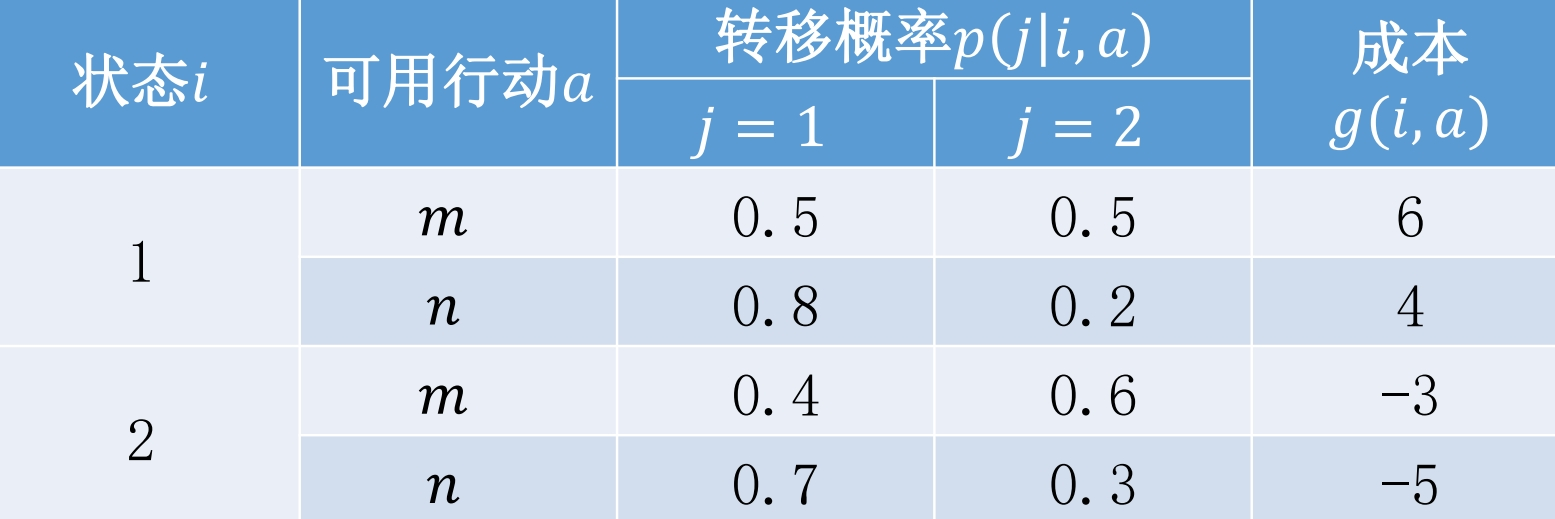
\includegraphics[scale=0.15]{pic/1.3.1.png}
        \caption{状态转移概率和成本函数}
    \end{figure}

    这时由4个平稳策略:
    \begin{equation}
        \begin{aligned}
            u_1 & = \{m,m\} \\
            u_2 & = \{m,n\} \\
            u_3 & = \{n,m\} \\
            u_4 & = \{n,n\} \\
        \end{aligned}
    \end{equation}

    先选择一个初始策略$u_1$,计算$J_1$:
    \begin{equation}
        \begin{aligned}
            6 + 0.9(0.5J_1 + 0.5J_2)  & = J_1 \\
            -3 + 0.9(0.4J_1 + 0.6J_2) & = J_2 \\
        \end{aligned}
    \end{equation}
    解的结果为$J_1(u_1) = 15.49 , J_2(u_1) = 5.60$。

    策略改善:对于状态$1$
    \begin{equation}
        \max \{g(1,a) + 0.9 \sum_{s\in S}p(j|1,a) J_s(u_1)\} = \max \begin{bmatrix}
            0.9(0.5J_1+0.5J_2) + 6 \\
            0.9(0.4J_1+0.6J_2) +4  \\
        \end{bmatrix} = 16.16
    \end{equation}
    采取行为$n$更优。

    对于状态$2$
    \begin{equation}
        \max \{g(2,a) + 0.9 \sum_{s\in S}p(j|2,a) J_s(u_1)\} = \max \begin{bmatrix}
            0.9(0.4J_1+0.6J_2) - 3 \\
            0.9(0.7J_1+0.3J_2) - 5 \\
        \end{bmatrix} = 6.27
    \end{equation}
    采取行为$n$更优。

    改进后的策略为$u_4 = \{n,n\}$。

    继续迭代还是收敛到$u_4$,最优值为$(22.20,12.31)$。
\end{example}

策略迭代的步骤2求解时将需要大量的计算,而异步策略迭代则可以避免这种情况。

其算法如下:

\begin{enumerate}[itemsep=0pt,parsep=0pt]
    \item 以策略$u_0$,$k=0$开始;
    \item 对于子集$s_k\in S$, 执行下面两步骤之一:
          \begin{enumerate}[itemsep=0pt,parsep=0pt]
              \item 数值更新:计算$J_{k+1} = T_{u_k}J_k$;
              \item 策略更新:选择$u_{k+1} = u_{J_{u_k}}$;
          \end{enumerate}
    \item 如果$u_{k+1} = u_k$,则停止,否则令$k=k+1$,转到步骤2。
\end{enumerate}

